\documentclass[prez_parietal.tex]{subfiles}
\begin{document}


%========================================================================
\section{Studying physiological signals}
%========================================================================
%------------------------------------------------------------------------
\subsection{Motivations}
%------------------------------------------------------------------------

\begin{frame}{Context}
		\vskip1em
		Collaboration with the Cognac-G laboratory:\\[1em]
		\begin{itemize}\itemsep2em
			\item Started in 2014
			\item Gathers MDs and mathematicians
			\item Goal:\\[1em] 
		\end{itemize}
		\bimplies{Quantification of human and animal phenome (behavior, movement,\dots).}
		\vskip1em
		{
		\centering
		\includegraphics[height=3em]{logo_cognac}\hspace{2em}
		\includegraphics[height=3em]{logo_sante_armees}\hspace{2em}
		
\includegraphics[height=3em]{logo_cnrs}\hspace{2em}
		
\includegraphics[height=2em]{logo-parisdescartes}\\
		}
\end{frame}


\begin{frame}{Signals from human walking}
	\centering
	\vskip1em
	\begin{tabular}{m{8em} m{20em}}
		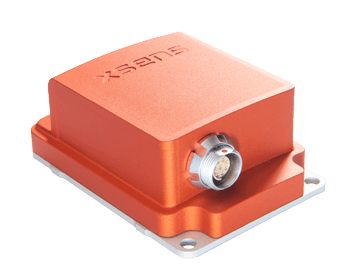
\includegraphics[width=.3\textwidth]{xsens} &
		\textbf{Properties}
		\begin{itemize}\itemsep-.2em
            \item Routine test
            \item Standardized protocol
            \item Signal with 24 channels (4x6)
            \item Minutes of signal recorded at 100Hz ($10^4$ samples)
		\end{itemize}
   \end{tabular}
	\centering
	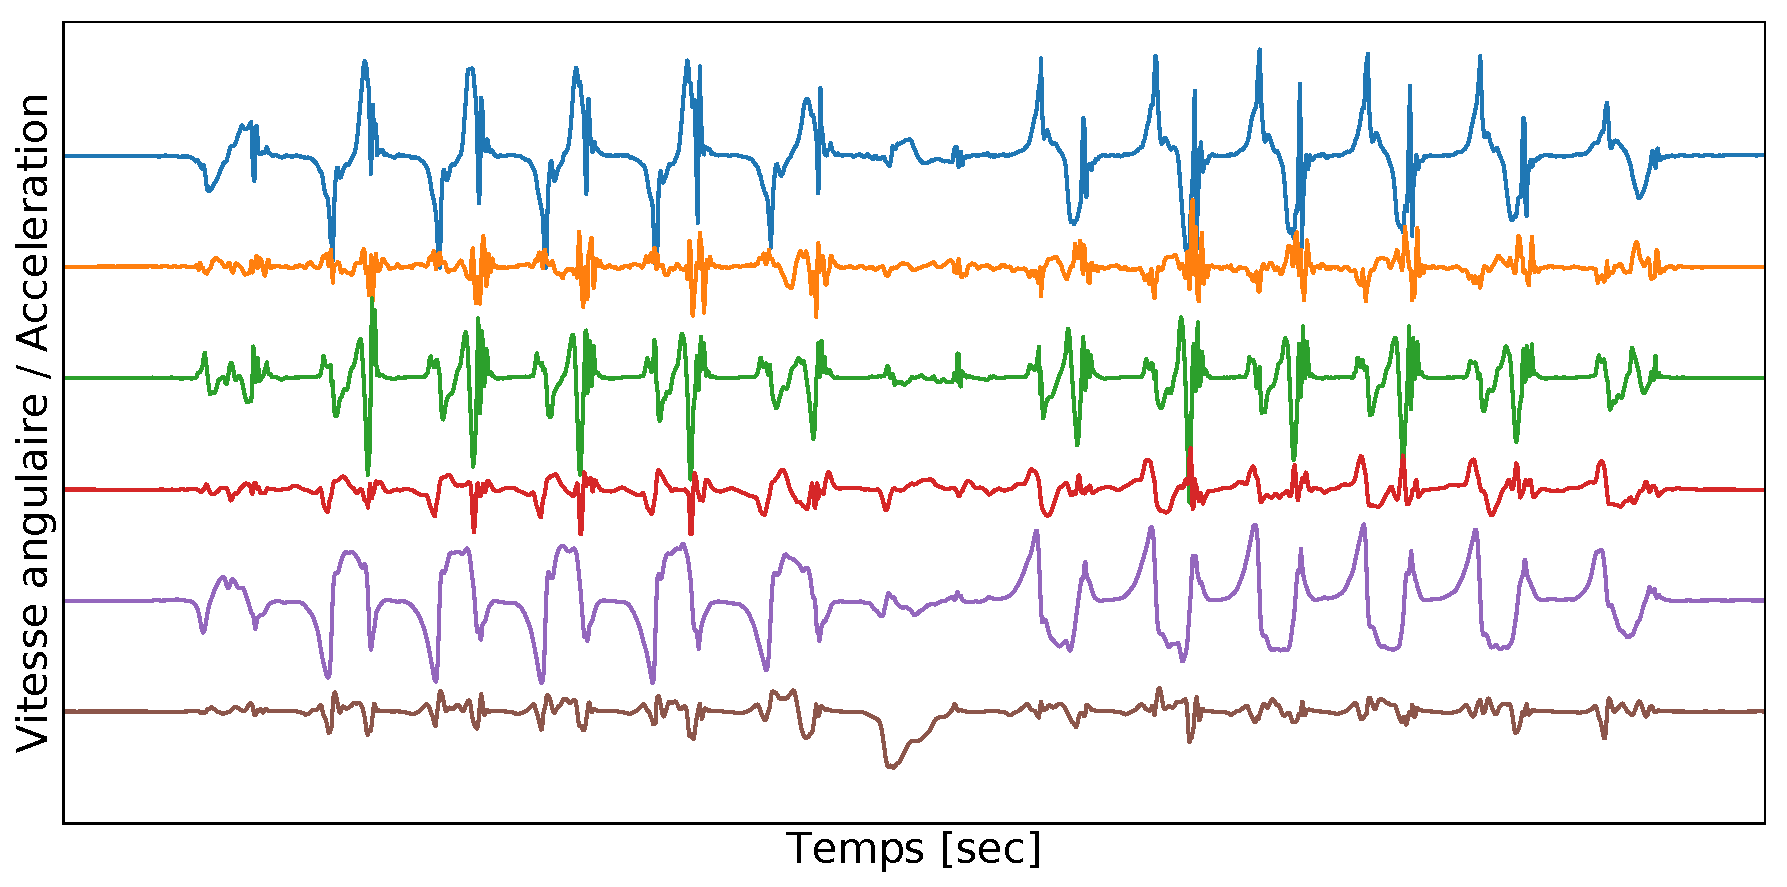
\includegraphics[width=.8\textwidth]{accelero}\\

\end{frame}
\begin{frame}{Automatized Analysis}

\begin{columns}[T]
\column{.4\textwidth}

		\btitle{Requirements\\[2em]}
		\begin{itemize}\itemsep1em
			\item Automatized analysis
			\item Robustness on a large basis
			\item Quick results
			\item Interpretability
		\end{itemize}
\column{.6\textwidth}
	\btitle{Challenges\\[2em]}
	\begin{itemize}\itemsep1em
		\item High-variability:\\
		\hskip2.5em{\small Healthy, Parkinsonian, Strokes,...}
		\item Non-stationary:\\
		\hskip2.5em{\small Multiple exercises in one signal}
		\item Need interpretability:\\
		\hskip2.5em{\small Link to medical analysis}
		\item Possibly long signals:\\
		\hskip2.5em{\small Ambulatory studies}
	\end{itemize}
\end{columns}
	%\vskip4em

\end{frame}

%------------------------------------------------------------------------
\subsection{Convolutional representations}
%------------------------------------------------------------------------

\begin{frame}[t]
	\frametitle{Notation}
	\begin{itemize}\itemsep1em
		\item $X$ is a signal of length $T$
		\item $\mathcal E$ is a noise signal of length $T$ 
		\item $\pmb D$ is a set of $K$ patterns of length $W$
		\item $Z$ is a signal of length $L = T-W+1$ in $\Rset^K$ 
	\end{itemize}
\vskip1em
{\bf Sparse Convolutional model:}
	\begin{align*}
		X[t] & = \sum_{k=1}^K (\pmb D_k*Z_k)[t] + \mathcal E[t]
	\end{align*}
	\vskip.5em
	with \makebox[1em]{$Z$} sparse. {\color{gray} Few of its coefficients are non-zero.}
\end{frame}
\begin{frame}[t]
	\frametitle{Model}
	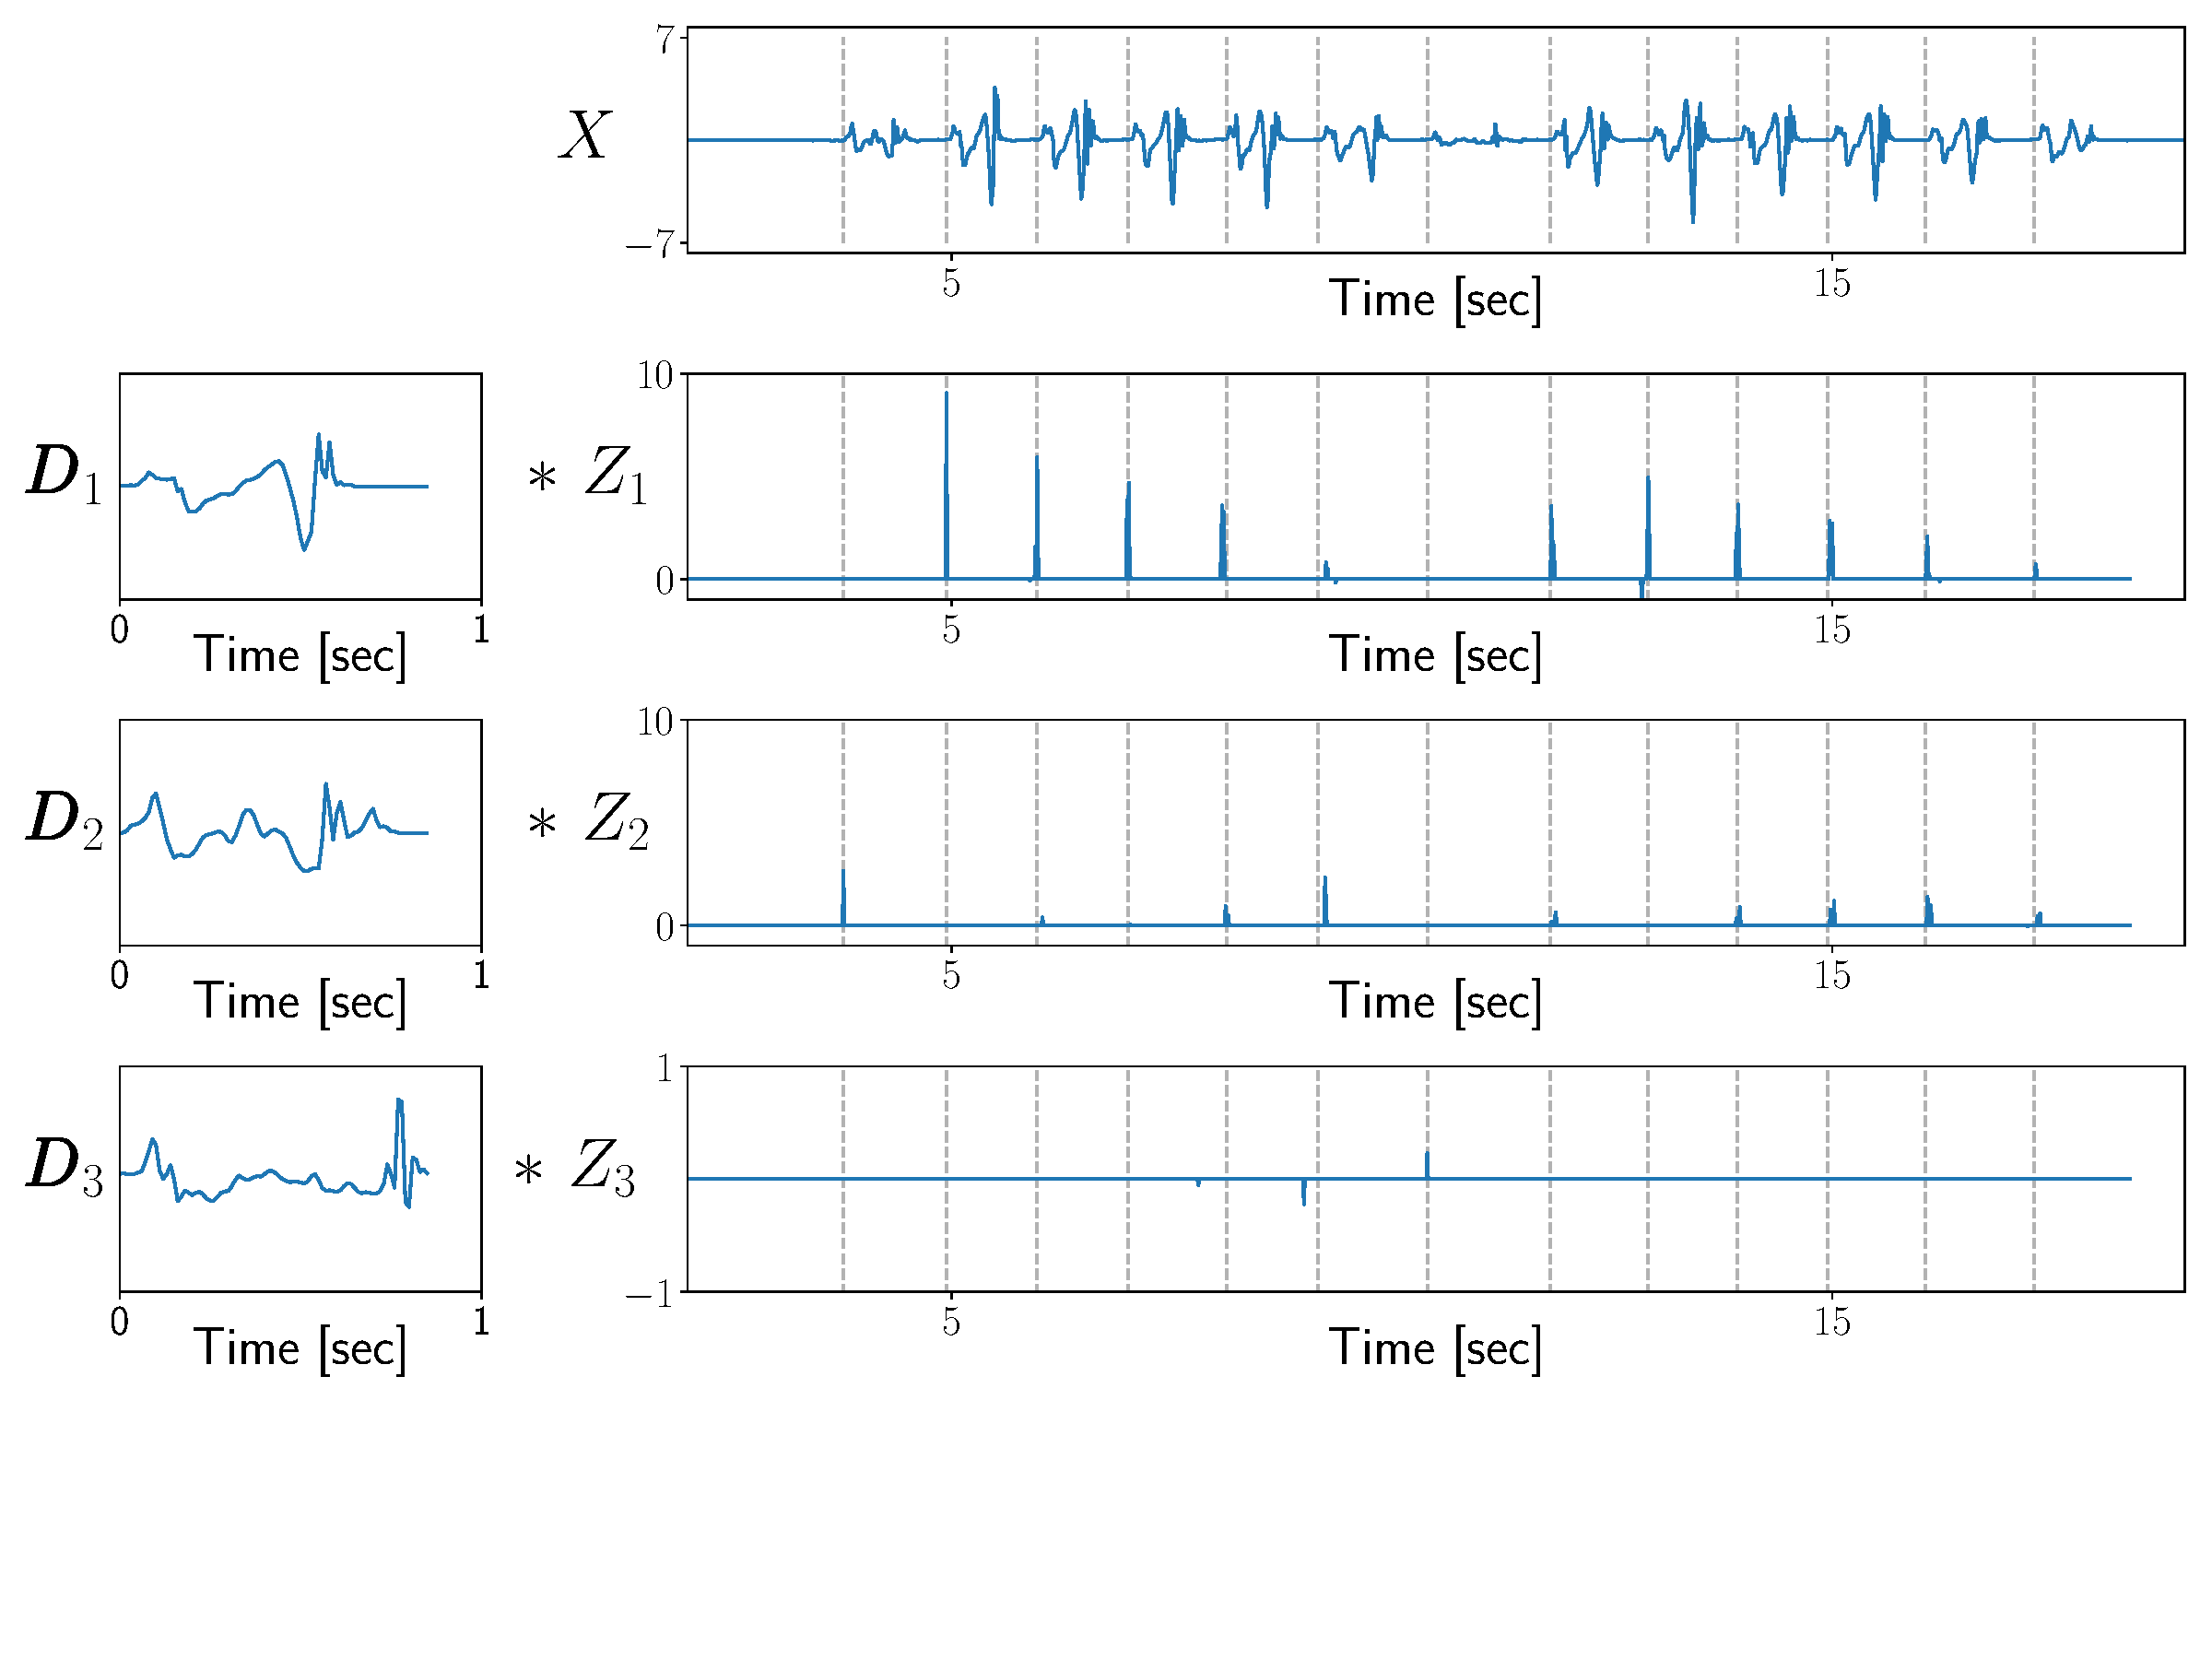
\includegraphics[width=.9\textwidth]{csc_explain}
\end{frame}

\begin{frame}[t]
	\frametitle{Vectorized model}
	\begin{columns}
	\column{.5\textwidth}
	\begin{itemize}\itemsep1em
		\item $x$ is a vector in $\Rset^T$
		\item $\epsilon$ is a noise vector in $\Rset^T$  
		\item $D$ is a matrix in $\Rset^{T\times LK}$
		\item $z$ is a coding vector in $\Rset^{LK}$ 
	\end{itemize}
	\column{.5\textwidth}
	{\bf Sparse Linear model:}
	\begin{align*}
		x & = Dz + \epsilon \phantom{ \sum_{k=1}^K }
	\end{align*}
	\vskip.5em
	with \makebox[1em]{$z$} sparse.\\{\color{gray} Few of its coefficients are non-zero.}
	\end{columns}
	\vskip1em
	\scriptsize\centering
	\inputTikZ{.4}{vectorial_dictionary}.\\
\end{frame}


%------------------------------------------------------------------------
\subsection{Convolutional dictionary Learning}
%------------------------------------------------------------------------
\begin{frame}[t]
\frametitle{Convolutional Sparse Model}
Dictionary learning optimization problem for $\{X^{[n]}\}_{n=1}^N$ 
\[\hskip-2em\begin{split}
	(Z^*, \pmb D^*) = \argmin_{Z, \pmb D}\frac{1}{N}\sum_{n=1}^N
			\underbrace{\| X^{[n]} - \sum_{k=1}^K\pmb D_k *  Z_k^{[n]}\|_2^2
						}_{E(Z) \text{ data fit}}\\
			+ \underbrace{\lambda\| Z^{[n]}\|_1 + \textbf{1}_{\Omega}(D)
						}_{\text{penalizations}}
\end{split}\]
with a constraint set $\Omega$ and a regularization parameter $\lambda > 0$.\\[1em]
This problem is non-convex and is generally solved using an \textbf{alternate minimization}.\\[.5em]
\mycite{Engan1999, Grosse2007}
\end{frame}

\begin{frame}[t]
\frametitle{$\pmb D$-step: Dictionary updates}
$\rightarrow Z$ fixed, update $\pmb D$
\[
	\pmb D^* = \argmin_{\pmb D}\frac{1}{N}\sum_{n=1}^N
			\| X^{[n]} - \sum_{k=1}^K\pmb D_k *  Z_k^{[n]}\|_2^2
				+ \textbf{1}_{\Omega}(D)
\]
\vskip1.5em
%
\underline{\textbf{Related Algorithms:}}\\[.5em]
\begin{itemize}\itemsep.5em
	\item Proximal Gradient Descent (PDG) \mycite{Rockafellar1976}
	\item Accelerated PGD \mycite{Nesterov1983}
	\item Block Coordinate Descent \mycite{Mairal2010}
	\item Alternated Direction Method of Multiplier (ADMM)\\\mycite{Gabay1976}
\end{itemize}
\end{frame}

\begin{frame}[t]
%\vskip-1em
\frametitle{$Z$-step: Sparse coding}
$\rightarrow \pmb D$ fixed, update $Z$
\[
	Z^{[n],*} = \argmin_{Z^{[n]}}\| X^{[n]} - \sum_{k=1}^K\pmb D_k *  Z_k^{[n]}\|_2^2
			+ \lambda\| Z^{[n]}\|_1
\]
\bimplies{Independent for each $n\in\llbracket1, N\rrbracket$}
\vskip1em
%
\underline{\textbf{Related Algorithms:}}\\[.5em]
\begin{itemize}%\itemsep.5em
	\item Iterative Soft-Thresholding Algorithm (ISTA)\\\mycite{Daubechies2004}
	\item Fast ISTA \\\mycite{Beck2009}
	\item Alternated Direction Method of Multiplier (ADMM)\\\mycite{Gabay1976}
	\item Coordinate Descent (CD) \\\mycite{Friedman2007}
\end{itemize}

	
\end{frame}

%\begin{frame}
%	\frametitle{Coordinate Descent \mycite{Friedman2007}}
%	{
%	\vskip2em
%	Select a coordinate $(k, t)$ and update it to the value
%	\[
%		Z_k'[t] = \argmin_{Z_k[t]}\| X - \sum_{k=1}^K\pmb D_k *  Z_k\|_2^2
%				+ \lambda\| Z\|_1
%	\]
%	with all other coordinates fixed.
	
%	\vskip2em
%	\centering
%	\inputTikZ{1}{cd_tikz}
%	}{ISTA \mycite{Daubechies2004}}{
%	\vskip2em
%	Proximal Gradient descent for Sparse Coding:
%	\[
%		Z^{(q+1)} = \text{Sh}\left(Z^{(q)} - \alpha\nabla E(Z^{(q)}), \alpha\lambda\right)
%	\]
%	with Sh$(Z_k[t], \lambda) = \text{sign}(Z_k[t])\max(|Z_k[t]|-\lambda, 0)$.

%	\vskip2em	
%	\centering
%	\inputTikZ{1}{pgd_tikz}
%	}
%\end{frame}


%---------------------------------------------------------------------------
\subsection{Accelerating the sparse coding}
%---------------------------------------------------------------------------

\begin{frame}
\frametitle{Part I: Distributed Coordinate Descent}

	Coordinate descent only update one coordinate at each iteration.\\[.5em]
	{\centering {\usebeamercolor[fg]{block title}$\Rightarrow$} Not efficient for convolutional model.\\[1.5em]}
	

	We could update $M$ coefficients in {\bf parallel}.\\[1.5em]
	
	{\bf General Parallel Coordinate Descent:}\\[.5em]
	\begin{itemize}\itemsep.5em
		\item Synchronous: \citet{Scherrer2012}, \citet{Bradley2011}.
		\item Asynchronous: \citet{Yu2012}, \citet{Low2012}.
	\end{itemize}

	\vskip1em
	\bf Can we do better with the structure of our problem?

\end{frame}

\begin{frame}{Part II: Adaptive Optimization}

	\vskip2em
	We have to solve $N$ independent problems with a common structure $\pmb D$,\\[.5em]
	\[
		Z^{[n],*} = \argmin_{Z^{[n]}}\| X^{[n]} - \sum_{k=1}^K\pmb D_k *  Z_k^{[n]}\|_2^2
				+ \lambda\| Z^{[n]}\|_1
	\]\vskip2em
	{\textbf{Can we use this structure to accelerate the resolution?}\\[1em]}
	\visible<2->{
		Yes, with the Learned ISTA. \mycite{Gregor10}\\[1em]
		%
		\textbf{Why does it work?}\\
	}
\end{frame}



\biblio{}
\end{document}